% XCircuit output "geometria.tex" for LaTeX input from geometria.eps
\def\putbox#1#2#3#4{\makebox[0in][l]{\makebox[#1][l]{}\raisebox{\baselineskip}[0in][0in]{\raisebox{#2}[0in][0in]{\scalebox{#3}{#4}}}}}
\def\rightbox#1{\makebox[0in][r]{#1}}
\def\centbox#1{\makebox[0in]{#1}}
\def\topbox#1{\raisebox{-0.60\baselineskip}[0in][0in]{#1}}
\def\midbox#1{\raisebox{-0.20\baselineskip}[0in][0in]{#1}}
   \scalebox{1}{
   \normalsize
   \parbox{3.79167in}{
   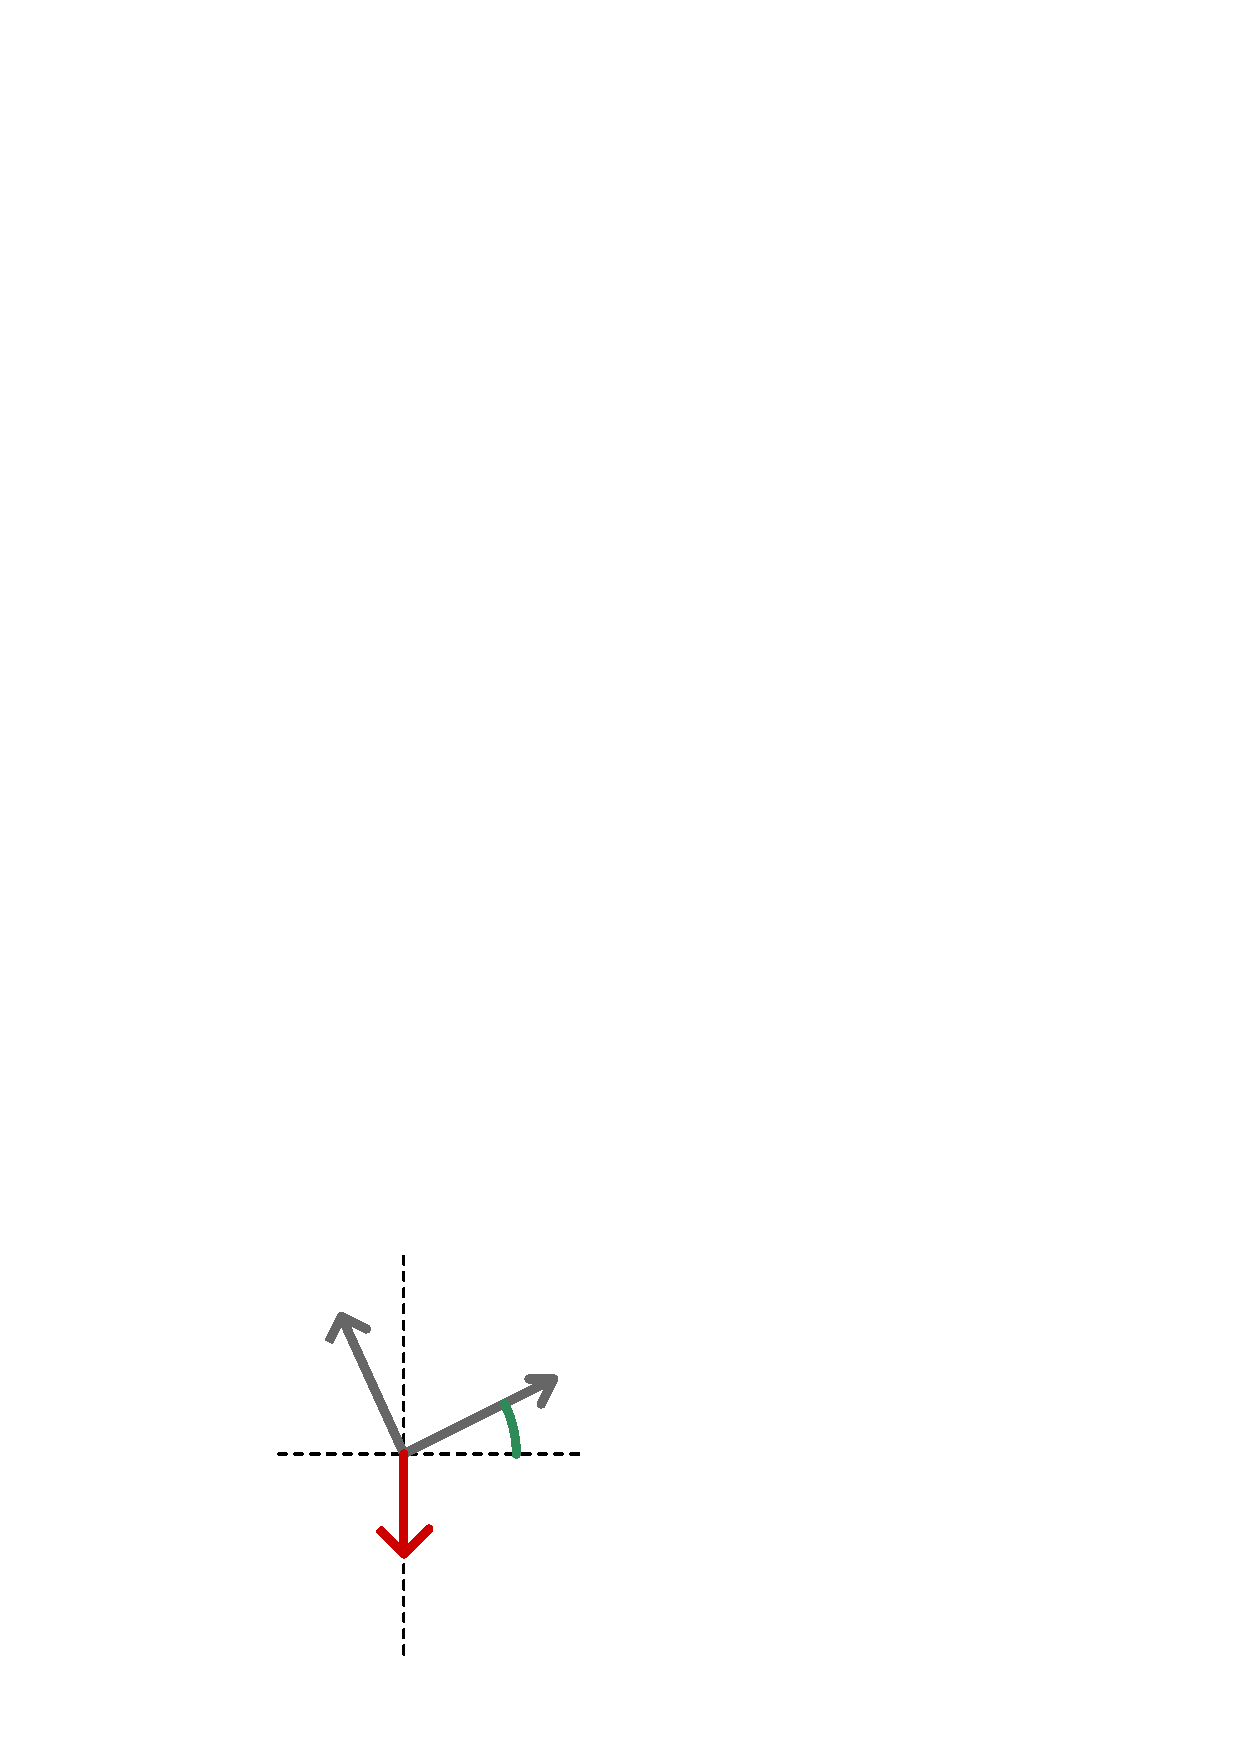
\includegraphics[scale=1]{geometria}\\
   % translate x=517 y=384 scale 0.38
   \putbox{2.58in}{1.72in}{1.20}{\rotatebox{-360}{\centbox{\midbox{{{$a_x$}}}}}}%
   \putbox{1.25in}{2.14in}{1.20}{\centbox{\midbox{$a_y$}}}%
   \putbox{1.58in}{0.72in}{1.20}{\rightbox{{\color{myred} $g$}}}%
   \putbox{2.75in}{1.14in}{1.20}{\centbox{{\color{mygreen} $\theta$}}}%
   } % close 'parbox'
   } % close 'scalebox'
   \vspace{-\baselineskip} % this is not necessary, but looks better
